\documentclass[../dissertation.tex]{subfiles}

\begin{document}

\subsection{Experiment 4 - Effects of Wi-Fi Connection}
\label{exp-4}

\paragraph{Introduction} Experiments 1, 2, and 3 were all conducted using a wired (Ethernet) connection from each of the Raspberry Pis to the router. This is optimal for communication performance as Ethernet is generally significantly faster than a wireless (Wi-Fi) connection, and is also significantly stabler - meaning that less packets become corrupted during sending, and therefore don't need to be sent multiple times. Wi-Fi is also much more susceptible to interference from other devices. However Wi-Fi does have the advantage of physical freedom of movement. In a multi-robot system it is reasonable that it would be advantageous (or even a requirement) for each robot to be physically mobile, thus in some cases it may be unavoidable to use Wi-Fi.

Given that it is plausible for a multi-robot system to use Wi-Fi as it's communication channel (the robot car platform described in Section \ref{background-robot-config} only supports Wi-Fi as physical access to the Ethernet ports is not possible), it is important to understand how Wi-Fi communication will affect performance compared to the ideal wired situation.

\paragraph{Objective} Experiment 4 investigates the effect of using a Wi-Fi network connection for message passing experiments. The target robot car platform described in Section \ref{background-robot-config} employ a Wi-Fi connection, thus understanding the effect this will have on the communication performance is required to understand the final performance of the system.

\paragraph{Hypothesis} The hypothesis was that switching to Wi-Fi would increase message latencies across all frequencies, and also reduce the maximum frequency that message latency remains consistent across the entire message stream (as in the previous experiment described in Section \ref{experiment3-cpu-speed}).

\paragraph{Materials and Methodology} The hardware platform (Raspberry Pi 3 Model B) utilised in these experiments contains Broadcom 802.11n WiFi chips which support a 2.4GHz network connection. This should give the Raspberry Pis an average data throughput of 25 Mbps, according to Cisco data\cite{florwick2013wireless}.

The experiment consists of running the same code in both wired (Ethernet) and wireless (Wi-Fi) settings. As before, the code will send timestamped messages from the sender host to the echoer host, which will send it back to the sender. The sender then records the message ID and sent and received times to file. The code is run 3 times with a range of message frequencies from 200Hz to 2000Hz in 200Hz steps (200Hz, 400Hz, ..., 1800Hz, 2000Hz) to obtained averaged results for each message frequency.

\paragraph{Results and Discussion} The experimental results after 3 runs in each setup appeared to mostly agree with the hypothesis. Overall message latencies were higher (as expected) across all frequencies using WiFi except 2000Hz - as shown in Figure \ref{exp4-means-all-freq}.

Figures \ref{exp4-ethernet-all-freq} and \ref{exp4-wifi-all-freq} demonstrate averages across 3 runs for all frequencies of the message streams, for Ethernet and WiFi respectively. \textit{It is clear from these figures that WiFi gives more erratic results than Ethernet, as well as overall lower performance, and thus it's effects must be carefully considered when using WiFi in future experiments.}

\begin{figure}[H]
\centering
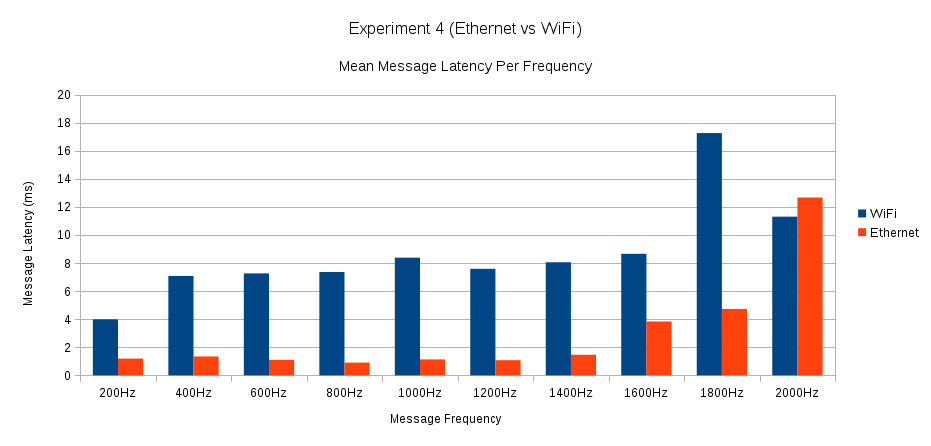
\includegraphics[width=\textwidth]{images/experiment4/mean_per_frequency.png}
\caption{Experiment 4 - Ethernet, All Frequencies}
\label{exp4-means-all-freq}
\end{figure}

\begin{figure}[H]
\centering
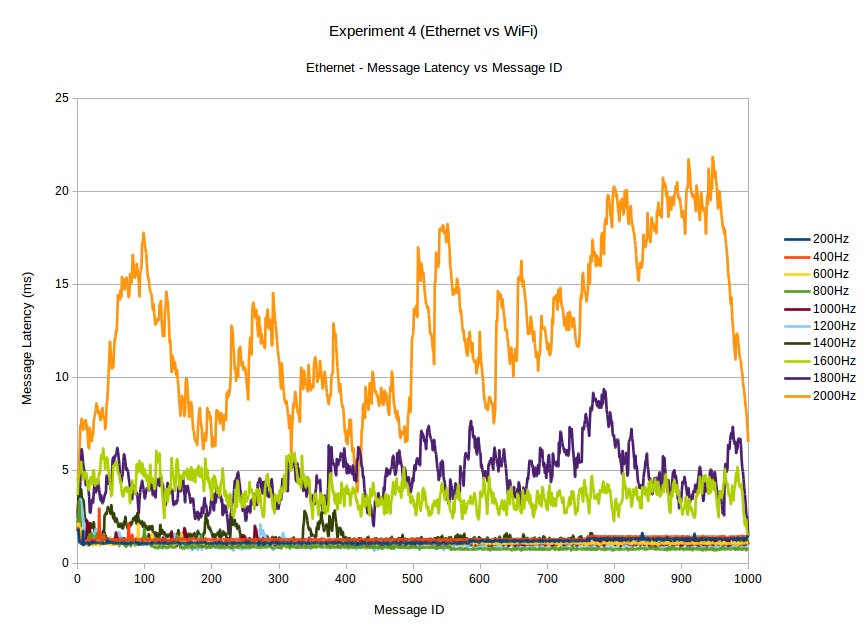
\includegraphics[width=\textwidth]{images/experiment4/ethernet_mean_times_pretty.png}
\caption{Experiment 4 - Ethernet, All Frequencies}
\label{exp4-ethernet-all-freq}
\end{figure}

\begin{figure}[H]
\centering
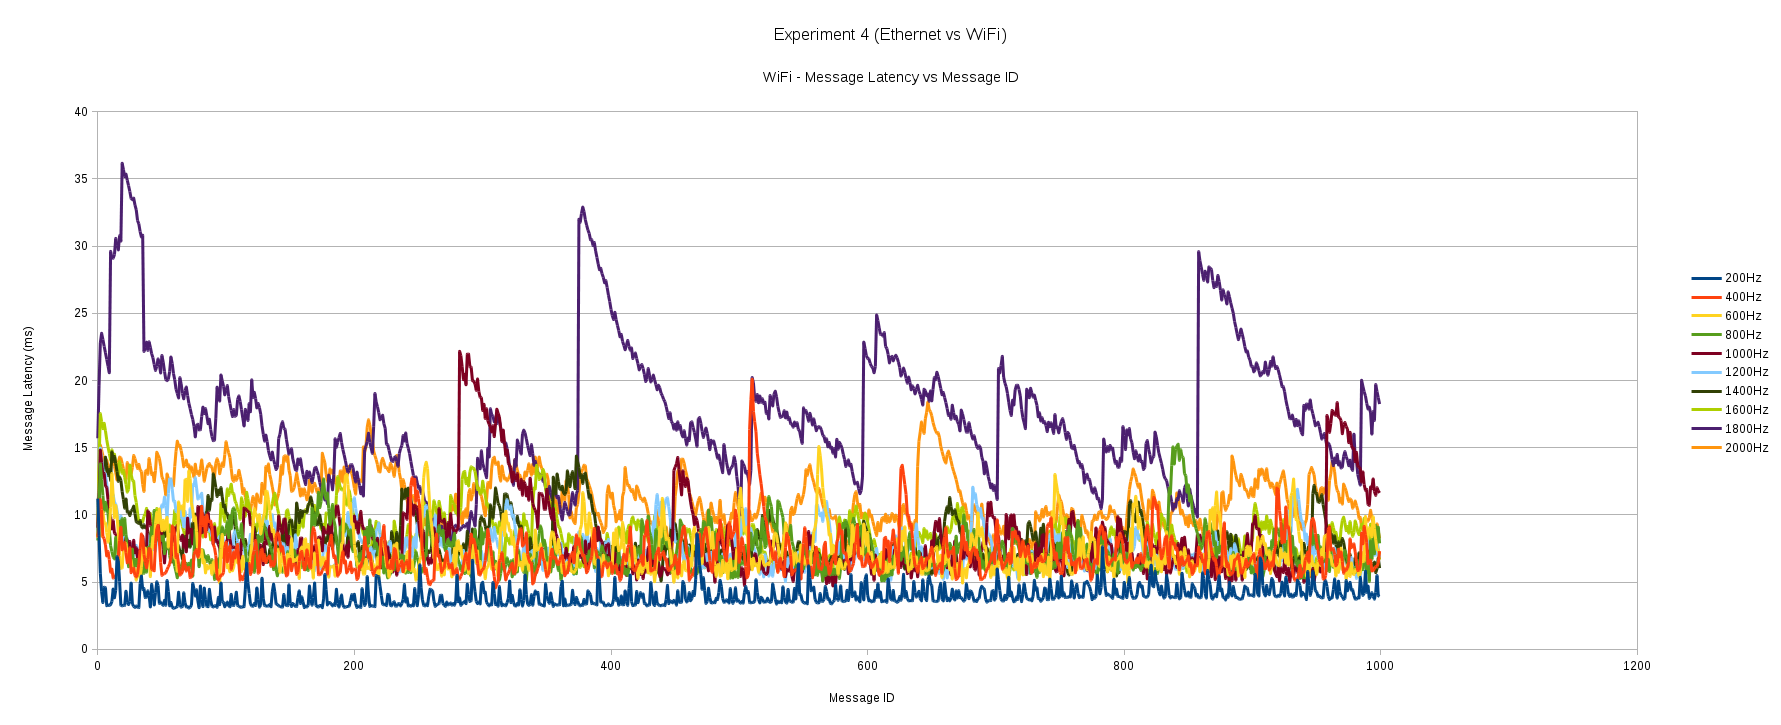
\includegraphics[width=\textwidth]{images/experiment4/wifi_mean_times_pretty.png}
\caption{Experiment 4 - Wi-Fi, All Frequencies}
\label{exp4-wifi-all-freq}
\end{figure}

\end{document}
